\chapter{Datasets Used and External Data Sources}

\section{Overview of Data Sources: What Information Lucid Uses}
To make intelligent investment recommendations, a financial system needs reliable, up-to-date information about companies, market prices, and the broader economy. Just as a human investor reads newspapers, reviews company annual reports, and checks stock exchange prices, Lucid collects data from verified official sources.

Lucid relies on five primary categories of data:
\begin{enumerate}
    \item \textbf{Stock Exchange Directories (NSE and BSE)}: The official registers of actively traded companies in India, including company names, exchange ticker symbols, and unique international identification numbers (called \textbf{ISINs}).
    \item \textbf{Historical Market Prices}: Daily trading prices (Open, High, Low, Close, and Volume) over the past 252 trading sessions (one full year) for every listed company.
    \item \textbf{Corporate Financial Fundamentals}: Vital balance sheet health metrics retrieved from quarterly financial reports, such as Return on Equity (ROE), Debt-to-Equity ratios, and Price-to-Earnings (P/E) ratios.
    \item \textbf{Macroeconomic Benchmarks from the Reserve Bank of India (RBI)}: Crucial national economic numbers, including the official RBI policy repo rate (6.50\%), inflation rates, and 10-year Indian government bond yields.
    \item \textbf{Financial News and Corporate Announcements}: Curated headlines and articles from recognized Indian business publications to identify company developments, legal risks, or management changes.
\end{enumerate}

Figure~\ref{fig:api_to_agent} illustrates how raw external information is downloaded, cleaned, stored in PostgreSQL, and converted into structured summaries for the AI agents:

\clearpage
\begin{figure}[p]
    \centering
    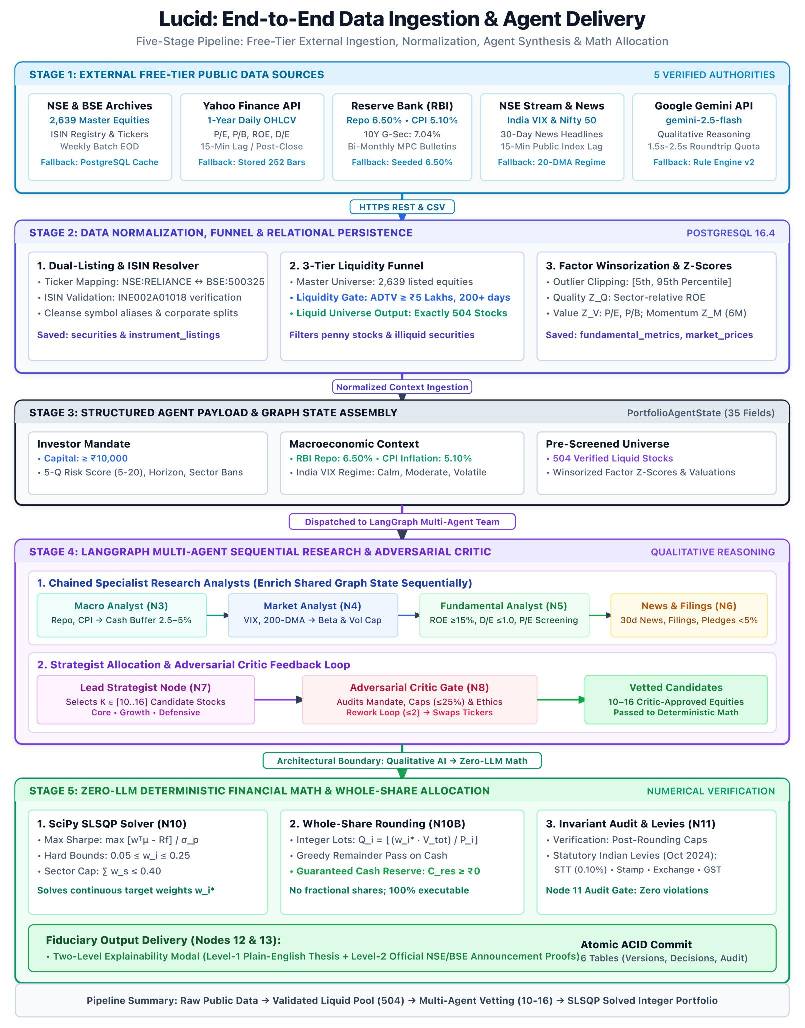
\includegraphics[width=0.92\textwidth, height=0.82\textheight, keepaspectratio]{API_TO_AGENT_DATA_FLOW.pdf}
    \caption{Data Ingestion, Transformation, and Agent Payload Delivery Pipeline}
    \label{fig:api_to_agent}
\end{figure}
\clearpage

\section{Inventory of External Data Sources}
Table~\ref{tab:external_data_sources} provides a comprehensive overview of every external data source integrated into Lucid, explaining what information is retrieved, how often it is refreshed, and what fallback safety measure is used if a provider is temporarily unavailable:

\begin{table}[H]
\centering
\caption{Lucid External Data-Source Inventory and Ingestion Parameters}
\label{tab:external_data_sources}
\resizebox{\textwidth}{!}{%
\begin{tabular}{lllll}
\toprule
\textbf{Data Source / Authority} & \textbf{Data Retrieved} & \textbf{Update Frequency} & \textbf{Primary Purpose} & \textbf{Offline Fallback Safety} \\
\midrule
\textbf{National Stock Exchange (NSE)} & Active stock list, ISINs, and tickers & Weekly / On Demand & Security master catalog & Cached PostgreSQL records \\
\textbf{Bombay Stock Exchange (BSE)} & Dual-listed company tickers and scrip codes & Monthly & Cross-exchange ticker mapping & Primary NSE ticker records \\
\textbf{Yahoo Finance (\texttt{yfinance})} & 1-Year daily price bars (OHLCV) & Daily after 16:30 IST & Volatility and covariance matrix & Stored historical price database \\
\textbf{Yahoo Finance Fundamentals} & P/E, P/B, ROE, Debt/Equity, Market Cap & Weekly & Balance sheet health screening & Cached \texttt{fundamental\_metrics} \\
\textbf{Reserve Bank of India (RBI)} & Official Repo Rate, CPI Inflation & Bi-monthly (MPC meeting) & Macroeconomic regime score & Seeded 6.50\% baseline \\
\textbf{NSE Index Stream} & India VIX and Nifty 50 Index quotes & 15-Minute Delayed Feed & Market volatility tiering & Historical 20-day moving average \\
\textbf{Google Gemini API} & Qualitative analysis and thesis synthesis & On-Demand per request & Contextual reasoning & Deterministic rule fallbacks \\
\bottomrule
\end{tabular}%
}
\end{table}

\section{Exchange Universe Coverage and Synchronization}

\subsection{Why Unique Company Identification (ISIN) Matters}
In India, a single company can have different names and ticker symbols across different platforms. For example, Tata Consultancy Services is traded as \texttt{TCS} on the National Stock Exchange (NSE) and as scrip code \texttt{532540} on the Bombay Stock Exchange (BSE). Furthermore, companies occasionally split their shares or change their corporate names.

To prevent confusion and eliminate duplicate entries, Lucid uses the \textbf{International Securities Identification Number (ISIN)}. An ISIN is a globally standardized 12-character alphanumeric code (such as \texttt{INE467B01029} for TCS) that permanently and uniquely identifies a security, regardless of which exchange it is traded on or what nickname it has.

\subsection{Resolving Corporate Splits and Duplicate Codes}
When corporate actions occur, companies may update their ISINs. Lucid's synchronization service (\texttt{exchange\_universe\_sync.py}) includes automated conflict resolution logic (\texttt{ON CONFLICT (isin) DO UPDATE}):
\begin{itemize}
    \item When \textbf{Bajaj Finance Ltd.} underwent a stock split from a face value of Rs.~10 to Rs.~2, its ISIN changed from \texttt{INE296A01016} to \texttt{INE296A01024}. Lucid recognized the corporate event, updated the active security identifier, and preserved all previous historical price records seamlessly.
    \item Similar split events for \textbf{Dr.~Reddy's Laboratories} and \textbf{Hindustan Aeronautics Ltd. (HAL)} were handled automatically without creating orphan records or crashing the database.
\end{itemize}

\subsection{Scale of the Active Investment Universe}
As verified in PostgreSQL:
\begin{itemize}
    \item \textbf{Total Cataloged Listed Equities}: Exactly \textbf{2,639 listed Indian companies} stored in the \texttt{securities} table.
    \item \textbf{Total Exchange Trading Listings}: Exactly \textbf{2,715 trading listings} in the \texttt{instrument\_listings} table (including dual listings across the NSE and BSE).
    \item \textbf{Active Recommendation Eligibility}: All 2,639 listed equities are dynamically screened based on investor risk capacity, institutional liquidity thresholds, and price data freshness.
    \item \textbf{Complete Coverage for Search and Statement Diagnostics}: All 2,639 stocks are instantly searchable in the user interface and fully recognized when users upload monthly Demat CAS statements.
\end{itemize}

\section{Historical Price Data and Statistical Calculations}
To calculate investment risks and expected returns, Lucid analyzes 252 consecutive trading sessions (one standard financial year) stored in the \texttt{market\_prices} table:

\begin{enumerate}
    \item \textbf{Daily Logarithmic Returns}:
    Instead of simple percentage changes, quantitative finance uses logarithmic returns because they are additive across time:
    \begin{equation}
    r_{i,t} = \ln \left( \frac{P_{i,t}^{\text{adjusted}}}{P_{i,t-1}^{\text{adjusted}}} \right)
    \end{equation}
    where $P_{i,t}^{\text{adjusted}}$ is the closing stock price adjusted for any dividends or stock splits.
    \item \textbf{Covariance Matrix ($\mathbf{\Sigma}$)}:
    To measure how different stocks move in relation to one another, Lucid calculates the sample covariance matrix across all shortlisted candidates:
    \begin{equation}
    \Sigma_{ij} = \frac{1}{T-1} \sum_{t=1}^{T} (r_{i,t} - \bar{r}_i)(r_{j,t} - \bar{r}_j)
    \end{equation}
    To convert daily covariance into annual terms, the matrix is multiplied by the annual trading day factor ($\sqrt{252}$).
\end{enumerate}

\section{Data Delivery: Feeding Clean Information to AI Agents}
A foundational architectural rule in Lucid is that \textbf{raw, unstructured API data is never dumped directly into the AI language model}.

Dumping raw website data or huge JSON files into an AI prompt causes three serious problems:
\begin{enumerate}
    \item It wastes expensive AI context tokens.
    \item It significantly slows down response times for the end user.
    \item It overwhelms the AI model with irrelevant information, increasing the risk of hallucinated or inaccurate conclusions.
\end{enumerate}

Instead, Lucid acts as a strict filter. Backend Python services process, clean, and verify external market data first, packaging only the essential, relevant fields into compact JSON payloads for each specialist agent.

Table~\ref{tab:agent_payloads} lists the exact structured data delivered to each agent:

\begin{table}[H]
\centering
\caption{Exact Data Payloads Delivered to LangGraph Multi-Agent Nodes}
\label{tab:agent_payloads}
\resizebox{\textwidth}{!}{%
\begin{tabular}{lllp{6cm}}
\toprule
\textbf{Agent Node} & \textbf{Data Source} & \textbf{Raw Data Format} & \textbf{Exact Structured Fields Delivered to Agent} \\
\midrule
\textbf{Input Validator} & User Web Form & JSON Payload & \texttt{capital\_inr}, \texttt{risk\_category}, \texttt{time\_horizon\_years}, \texttt{goal\_name}, \texttt{excluded\_sectors} \\
\textbf{Macro Analyst} & RBI Policy Bulletins & HTML / Reports & \texttt{rbi\_repo\_rate\_pct}, \texttt{inflation\_cpi\_pct}, \texttt{gdp\_forecast}, \texttt{monetary\_stance} \\
\textbf{Market Regime} & NSE Index Streams & Live Quotes & \texttt{india\_vix\_value}, \texttt{vix\_tier}, \texttt{nifty\_current}, \texttt{nifty\_50\_dma}, \texttt{regime\_trend} \\
\textbf{Universe Selector} & PostgreSQL Master & SQL Records & Filtered candidates: \texttt{symbol}, \texttt{company\_name}, \texttt{sector}, \texttt{liquidity\_tier} \\
\textbf{Fundamental Analyst} & Yahoo Finance / DB & Balance Sheets & Per Candidate: \texttt{symbol}, \texttt{pe\_ratio}, \texttt{pb\_ratio}, \texttt{roe\_pct}, \texttt{debt\_to\_equity} \\
\textbf{News Analyst} & Curated Ingested News & Text Articles & Per Candidate: \texttt{symbol}, \texttt{headline\_count}, \texttt{sentiment\_score}, \texttt{legal\_risk\_flags} \\
\textbf{Adversarial Critic} & Preceding Agent State & Python Dictionary & Candidate shortlist, proposed sector weights, identified risk factors \\
\textbf{SLSQP Optimizer} & Quant Service & Math Arrays & Covariance matrix $\mathbf{\Sigma}$, expected returns $\boldsymbol{\mu}$, risk-free rate $R_f$, budget bounds \\
\textbf{Explainability Node} & Portfolio Decisions & DB Records & Final chosen symbols, allocated shares, weights, Sharpe score, risk contributions \\
\bottomrule
\end{tabular}%
}
\end{table}

\subsection{Example of a Sanitized Agent Payload}
Below is a real example of the clean, focused data package sent to the \textbf{Fundamental Analyst Agent}:

\begin{footnotesize}
\begin{verbatim}
{
  "macro_context": {
    "repo_rate": 6.50,
    "vix_tier": "Normal Volatility (14.2)",
    "market_trend": "Bullish above 200-DMA"
  },
  "candidate_stocks": [
    {
      "symbol": "TCS",
      "company": "Tata Consultancy Services Ltd.",
      "sector": "Information Technology",
      "pe_ratio": 28.4,
      "roe_pct": 46.2,
      "debt_to_equity": 0.08
    },
    {
      "symbol": "HDFCBANK",
      "company": "HDFC Bank Ltd.",
      "sector": "Financial Services",
      "pe_ratio": 18.9,
      "roe_pct": 16.8,
      "debt_to_equity": 1.12
    }
  ]
}
\end{verbatim}
\end{footnotesize}

By providing only verified, essential numbers, the AI agent can complete its evaluation quickly, reliably, and without confusion.
